
\subsection{Gradings}

\begin{figure}[H]
    \centering
    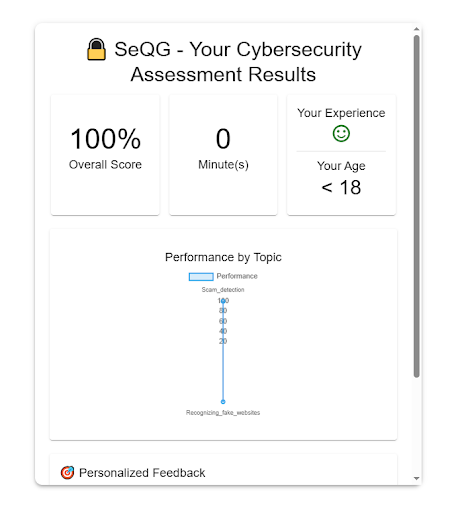
\includegraphics[width=0.4\textwidth]{images/Grading2.png}
    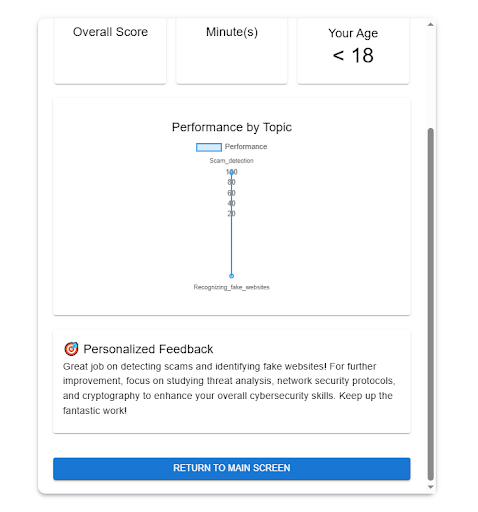
\includegraphics[width=0.4\textwidth]{images/Grading3.png}
    \caption{Dashboard}
\end{figure}
When the user finishes their session (in both guest and private modes), a dashboard appears summarizing their \textbf{performance}. 
To enhance user feedback and engagement in SeQG, the dashboard includes radar charts assessing the user's performance 
across each specific \textbf{cybersecurity topic}, generated with Chart.js. The diagram is split into two if there are more 
than eight topics, to avoid exceeding the visual limit. The dashboard also includes \textbf{personalized feedback}, as 
shown in Figure 2.5, which highlights the user's strengths and weaker areas during their session, encouraging 
them to use SeQG again to improve their \textbf{cybersecurity awareness}. User Progress is persistently stored in a 
structured JSON format if the user started a private session, including metadata such as their userID, age, 
experience and per-topic experience.


\begin{figure}[H]
    \centering
    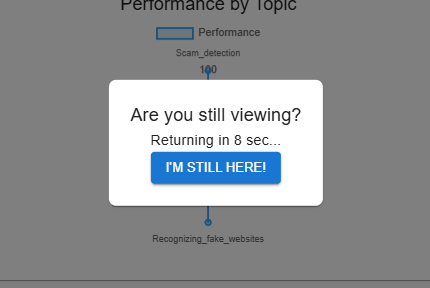
\includegraphics[width=0.35\textwidth]{images/Grading1.png}
    \caption{Inactivity timer pop-up message}
\end{figure}
The interface also includes an inactivity timer that triggers a message in the center of the screen after 60 seconds 
of \textbf{no interaction}. The user then has 10 seconds to confirm their presence; otherwise, the session is closed and the 
system returns to the main screen.